\chapter{Giới thiệu}
\label{chap:intro}

\section{Động lực nghiên cứu}
Khóa luận dùng nghiên cứu \emph{Longitudinal structural MRI-based deep learning and radiomics features for predicting Alzheimer's disease progression} của Aghajanian và cộng sự \cite{aghajanian2025longitudinal} làm công trình tham chiếu ban đầu để phát triển và so sánh phương pháp. Nghiên cứu đó phân tích ảnh chụp cộng hưởng từ cấu trúc T1 (MRI T1) ở nhiều thời điểm, dùng mạng nơ-ron CNN để rút đặc trưng từ ảnh, T-LSTM để xem sự thay đổi qua các lần chụp, cơ chế attention để mô hình tập trung vào thông tin quan trọng và mô hình sống còn để xếp hạng nguy cơ biến cố theo thời gian. Kết quả bài báo cho thấy việc thêm radiomics chưa giúp mô hình tốt lên một cách ổn định; vì vậy, khóa luận kiểm tra xem ảnh MRI, các đặc trưng số mô tả ảnh và thông tin lâm sàng nên được kết hợp với nhau như thế nào.

Bệnh Alzheimer (Alzheimer's disease -- AD) có thể làm trí nhớ, khả năng suy nghĩ và sinh hoạt hằng ngày suy giảm dần. Suy giảm nhận thức nhẹ (Mild Cognitive Impairment -- MCI) là tình trạng cần được theo dõi, bởi những người có cùng chẩn đoán ban đầu vẫn có thể diễn biến khác nhau: một số tiến triển thành sa sút trí tuệ, một số ổn định, còn một số cải thiện \cite{petersen2018mci,jack2018niaaa}. Vì thế, nhận biết người bệnh đang ở tình trạng nào và dự báo họ có thể diễn biến ra sao là hai việc khác nhau; khóa luận tập trung vào việc thứ hai, tức là dùng thông tin đã thu thập qua các lần khám để xếp hạng người nào có nguy cơ tiến triển sớm hơn.

Khi theo dõi một người qua nhiều lần khám, ta có thể xem cả tình trạng của họ lẫn những thay đổi xảy ra theo thời gian. MRI cấu trúc cho thấy hình ảnh giải phẫu não; radiomics chuyển hình dạng, độ sáng và kết cấu của ảnh thành các đặc trưng có thể đo lường; còn các thông tin lâm sàng mô tả khả năng nhận thức và sinh hoạt \cite{vangriethuysen2017computational}. Khi được ghép đúng cách, các nguồn thông tin này có thể bổ sung cho nhau, nhưng chúng cũng có thể lặp lại cùng một thông tin, khác thang đo hoặc chứa nhiễu; do đó, khóa luận kiểm tra lợi ích của việc kết hợp dữ liệu bằng thực nghiệm thay vì mặc định rằng càng có nhiều đầu vào thì mô hình càng tốt.

\section{Phát biểu bài toán}
Đề tài \emph{Longitudinal Learning with Tensor Fusion for Predicting Progression of Alzheimer's Disease} xây dựng mô hình dự báo nguy cơ tiến triển cho nhóm người bị MCI trong dữ liệu của Alzheimer's Disease Neuroimaging Initiative (ADNI) \cite{weiner2015impact}. Mỗi người có ba lần chụp MRI được chọn trong 18 tháng đầu kể từ lần khám ban đầu, cùng các đặc trưng radiomics và thông tin lâm sàng được ghép với từng lần chụp. Mô hình đưa ra một điểm nguy cơ liên tục: điểm càng cao thì nguy cơ tương đối theo mô hình càng lớn, nhưng đây không phải phần trăm khả năng mắc AD và cũng không phải chẩn đoán AD.

\begin{figure}[htbp]
\centering
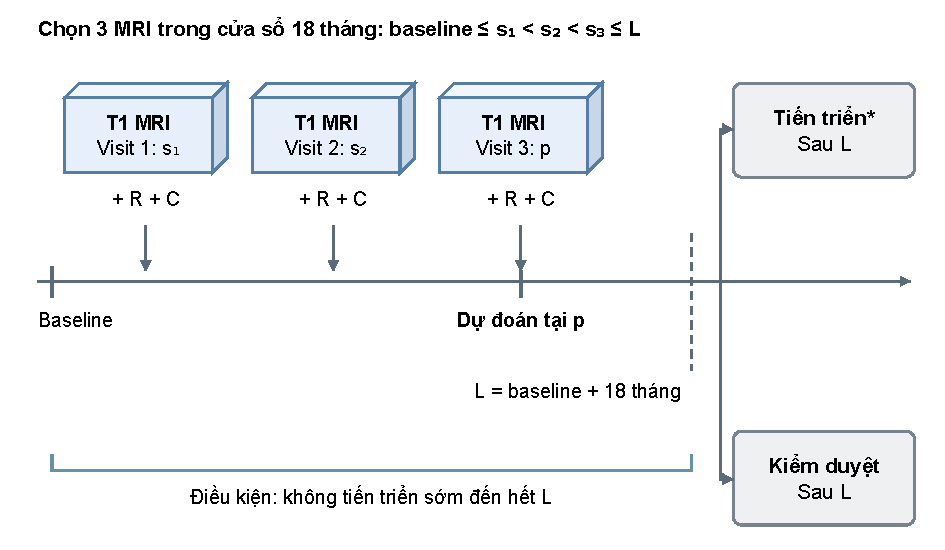
\includegraphics[width=\textwidth]{image/mci-progression-timeline.pdf}
\caption[Bài toán dự báo tiến triển MCI theo thời gian]{Sơ đồ chọn ba lần chụp MRI trong 18 tháng kể từ lần khám ban đầu. $L$ là ngày kết thúc khoảng thời gian này, bằng ngày khám ban đầu cộng 18 tháng theo lịch; đây là mốc quyết định người bệnh có được chọn vào nhóm nghiên cứu hay không. $p$ là ngày chụp MRI thứ ba và là mốc bắt đầu tính thời gian đến biến cố, nên $p\leq L$. Sau $L$, biến cố được ghi nhận khi MMSE $<24$ hoặc CDR-global $\geq1$; đây là tiêu chí dựa trên ngưỡng điểm, không phải chẩn đoán AD đã được xác nhận. $o$ là ngày xảy ra biến cố hoặc ngày theo dõi hợp lệ cuối cùng, và số năm theo dõi được tính bằng số ngày từ $p$ đến $o$ chia cho 365.25. Thông tin lâm sàng được ghép từ lần đo gần nhất trong vòng 90 ngày trước hoặc sau ngày MRI, nên đôi khi được thu thập sau khi chụp ảnh.}
\label{fig:problem-timeline}
\end{figure}

Hình~\ref{fig:problem-timeline} có hai mốc cần phân biệt. $L$ là ngày khép lại khoảng 18 tháng dùng để chọn nhóm nghiên cứu, còn $p$ là ngày chụp MRI thứ ba và là điểm bắt đầu tính thời gian đến biến cố; trong bộ dữ liệu này, $p\leq L$. Nói cách khác, $L$ quyết định ai được đưa vào nhóm nghiên cứu, còn $p$ cho biết mô hình bắt đầu tính thời gian từ ngày nào. Sau $L$, biến cố được ghi nhận ở lần đầu tiên người bệnh có MMSE $<24$ hoặc CDR-global $\geq1$; đây là \emph{dấu hiệu thay thế dựa trên điểm số}, chứ không khẳng định người đó đã được chẩn đoán AD hoặc đã được xác nhận bệnh bằng dấu ấn sinh học. Nếu người bệnh đạt một trong hai ngưỡng, chỉ báo biến cố $\delta=1$; nếu họ chưa đạt ngưỡng cho đến lần theo dõi hợp lệ cuối cùng, $\delta=0$ và dữ liệu được xem là chưa ghi nhận biến cố trong thời gian theo dõi. Vì vậy, $\delta=0$ không có nghĩa là người đó sẽ không tiến triển về sau.

Khóa luận phân tích dữ liệu đã được thu thập trước đó, và thông tin lâm sàng được ghép theo ngày gần nhất trong khoảng 90 ngày trước hoặc sau mỗi lần MRI. Vì khoảng ghép kéo dài cả về trước lẫn sau, một số thông tin có thể được ghi nhận sau ngày chụp MRI thứ ba; do đó, việc chia dữ liệu theo từng người và chỉ tính các bước tiền xử lý trên tập huấn luyện giúp hạn chế lẫn thông tin giữa các nhóm, nhưng chưa chứng minh rằng mọi đầu vào đều đã có sẵn đúng tại ngày $p$ nếu áp dụng mô hình trong thực tế. Chương~\ref{chap:method} mô tả cách ghép dữ liệu, còn Chương~\ref{chap:discussion} bàn thêm giới hạn này.

Về cách kết hợp dữ liệu, concatenation chỉ nối các nhóm đặc trưng cạnh nhau rồi để các lớp tiếp theo tự học mối liên hệ; còn phép tích ngoài (outer product) tính trực tiếp tương tác giữa từng cặp đặc trưng, nhưng số phép tính và tham số có thể tăng nhanh \cite{zadeh2017tensor}. Vì vậy, khóa luận lần lượt kiểm tra liệu có cần tạo tương tác riêng hay không, liệu có thể dùng phương pháp CP để biểu diễn gọn phần tương tác hay không, và liệu có cần giữ tương tác trực tiếp giữa mọi cặp dữ liệu hay không.

\section{Câu hỏi nghiên cứu}
Các câu hỏi trong Bảng~\ref{tab:rq} đi theo từng bước phát triển mô hình, và mỗi câu hỏi được gắn với một phép so sánh cụ thể. Kết quả chỉ phản ánh nhóm người bệnh và cách đánh giá được dùng trong khóa luận, nên không có nghĩa là một kiến trúc sẽ luôn tốt hơn trên mọi bộ dữ liệu.

Các thử nghiệm ban đầu lần lượt chuyển từ MRI đơn sang MRI theo thời gian, rồi kết hợp nhiều loại dữ liệu; tuy nhiên, trong quá trình thăm dò đó, một số phần khác như bộ trích đặc trưng, mô-đun xử lý chuỗi và cách chia batch cũng thay đổi. Vì vậy, không thể quy toàn bộ chênh lệch kết quả giữa các giai đoạn cho riêng việc thêm một loại dữ liệu hay đổi cách kết hợp; để đánh giá từng thành phần, khóa luận dựa nhiều hơn vào các phép so sánh chỉ thay đổi một yếu tố, các thử nghiệm lần lượt bỏ từng thành phần và bài đánh giá chuẩn hóa.

\begin{table}[htbp]
\centering
\caption{Câu hỏi nghiên cứu định hướng các thực nghiệm.}
\label{tab:rq}
\begin{tabularx}{\textwidth}{C{1.0cm}Y}
\toprule
\textbf{Mã} & \textbf{Câu hỏi nghiên cứu} \\
\midrule
RQ1 & Dùng nhiều lần MRI theo thời gian có giúp dự báo tốt hơn chỉ dùng MRI ở một lần khám trong nhóm nghiên cứu này không? \\
RQ2 & Khi nối các đặc trưng lại với nhau, radiomics và thông tin lâm sàng bổ sung được gì ngoài MRI? \\
RQ3 & Nếu giữ các phần khác của quy trình như nhau, tạo tương tác riêng giữa từng cặp dữ liệu có tốt hơn chỉ nối các đặc trưng không? \\
RQ4 & Dùng dạng CP để làm gọn phần tính tương tác giúp giảm số tham số đến đâu, và kết quả trên tập kiểm định thay đổi như thế nào? \\
RQ5 & Cổng điều tiết, hệ số của từng nhánh kết nối và nhánh giữ lại đặc trưng ban đầu đóng góp ra sao; có thể bỏ tương tác trực tiếp giữa radiomics và thông tin lâm sàng hay không? \\
\bottomrule
\end{tabularx}
\end{table}

\FloatBarrier
\section{Mục tiêu nghiên cứu}
Mục tiêu chung là xây dựng và phân tích một quy trình dùng nhiều lần khám cùng nhiều loại dữ liệu để dự báo tiến triển MCI, đồng thời chọn cách kết hợp dữ liệu dựa trên kết quả thử nghiệm. Cụ thể, khóa luận thực hiện các việc sau:
\begin{enumerate}
  \item Tạo nhóm người có đủ ba lần chụp MRI, xác định rõ tiêu chí ghi nhận biến cố và trường hợp chưa thấy biến cố; chia dữ liệu theo từng người và chỉ học bước chuẩn hóa từ tập huấn luyện.
  \item So sánh mô hình dùng một lần MRI, nhiều lần MRI theo thời gian và cả MRI, radiomics cùng thông tin lâm sàng để xem thời gian và mỗi loại dữ liệu bổ sung ích lợi gì.
  \item Tạo tương tác riêng giữa từng cặp MRI--radiomics, MRI--lâm sàng và radiomics--lâm sàng, rồi đưa các đặc trưng mới này trở lại mô hình bằng cơ chế điều tiết.
  \item So sánh cách tính đầy đủ các tương tác với cách biểu diễn gọn bằng CP, rồi lần lượt bỏ từng thành phần để xem thành phần nào thực sự cần thiết.
  \item Chọn mô hình dựa trên tập kiểm định, nhiều lần chạy với cách khởi tạo khác nhau và các bài đánh giá chuẩn hóa; giữ riêng tập đánh giá cuối cùng, không dùng tập này để chọn mô hình.
\end{enumerate}

\section{Đóng góp của khóa luận}
Đóng góp của khóa luận là xây dựng quy trình kết hợp dữ liệu và kiểm tra từng phần của mô hình trước khi chọn kiến trúc cuối:
\begin{enumerate}
  \item Kết hợp MRI 3D, radiomics và thông tin lâm sàng qua nhiều lần khám; T-LSTM theo dõi thay đổi theo thời gian, attention nhấn mạnh thông tin quan trọng, còn mô hình Cox dùng để xếp hạng nguy cơ biến cố.
  \item Tạo tương tác cho từng cặp dữ liệu, rồi đưa chúng trở lại mô hình qua cổng điều tiết phụ thuộc đầu vào và hệ số riêng cho mỗi nhánh. Ý tưởng có tham khảo các nghiên cứu về dùng cổng để giữ thông tin cũ và điều chỉnh mức đóng góp của thông tin mới, còn công thức cụ thể do khóa luận xây dựng \cite{ryumina2026residual,liu2026motion}.
  \item Dùng phương pháp CP, tức cách biểu diễn khối hệ số nhiều chiều (tensor trọng số) bằng các phần gọn hơn, để giảm số hệ số của lớp tương tác; cách này không phân rã dữ liệu của từng người bệnh.
  \item Chọn \textbf{RC-Free Pairwise Fusion} sau khi lần lượt bỏ từng thành phần để so sánh. Mô hình vẫn dùng đủ MRI, radiomics và thông tin lâm sàng, nhưng không tạo tương tác trực tiếp giữa radiomics và lâm sàng.
  \item So sánh các mô hình trên cùng cách chia dữ liệu qua ba lần chạy, rồi xem độ dao động kết quả và số tham số để cân nhắc giữa độ phức tạp với hiệu quả dự báo.
\end{enumerate}

CP được chọn sau khi so sánh, còn RC-Free được giữ lại sau khi thử bỏ từng thành phần và đối chiếu validation qua ba seed. Khóa luận báo cáo thêm test hậu nghiệm của các checkpoint đã chọn; các kết quả phản ánh nhóm nghiên cứu hiện tại, còn đánh giá cuối cùng trên cohort độc lập hoặc tập giữ lại mới chưa được thực hiện.

\section{Cấu trúc khóa luận}
Khóa luận gồm năm chương: Chương~\ref{chap:background} trình bày kiến thức nền về dự báo MCI, thời gian đến biến cố và kết hợp dữ liệu; Chương~\ref{chap:method} mô tả cách chọn người tham gia, xử lý dữ liệu và xây dựng mô hình. Chương~\ref{chap:results} trình bày các thí nghiệm và kết quả, còn Chương~\ref{chap:discussion} bàn về ý nghĩa, giới hạn, hướng phát triển và kết luận.
